
%% bare_jrnl.tex
%% V1.3
%% 2007/01/11
%% by Michael Shell
%% see http://www.michaelshell.org/
%% for current contact information.
%%
%% This is a skeleton file demonstrating the use of IEEEtran.cls
%% (requires IEEEtran.cls version 1.7 or later) with an IEEE journal paper.
%%
%% Support sites:
%% http://www.michaelshell.org/tex/ieeetran/
%% http://www.ctan.org/tex-archive/macros/latex/contrib/IEEEtran/
%% and
%% http://www.ieee.org/



% *** Authors should verify (and, if needed, correct) their LaTeX system  ***
% *** with the testflow diagnostic prior to trusting their LaTeX platform ***
% *** with production work. IEEE's font choices can trigger bugs that do  ***
% *** not appear when using other class files.                            ***
% The testflow support page is at:
% http://www.michaelshell.org/tex/testflow/


%%*************************************************************************
%% Legal Notice:
%% This code is offered as-is without any warranty either expressed or
%% implied; without even the implied warranty of MERCHANTABILITY or
%% FITNESS FOR A PARTICULAR PURPOSE!
%% User assumes all risk.
%% In no event shall IEEE or any contributor to this code be liable for
%% any damages or losses, including, but not limited to, incidental,
%% consequential, or any other damages, resulting from the use or misuse
%% of any information contained here.
%%
%% All comments are the opinions of their respective authors and are not
%% necessarily endorsed by the IEEE.
%%
%% This work is distributed under the LaTeX Project Public License (LPPL)
%% ( http://www.latex-project.org/ ) version 1.3, and may be freely used,
%% distributed and modified. A copy of the LPPL, version 1.3, is included
%% in the base LaTeX documentation of all distributions of LaTeX released
%% 2003/12/01 or later.
%% Retain all contribution notices and credits.
%% ** Modified files should be clearly indicated as such, including  **
%% ** renaming them and changing author support contact information. **
%%
%% File list of work: IEEEtran.cls, IEEEtran_HOWTO.pdf, bare_adv.tex,
%%                    bare_conf.tex, bare_jrnl.tex, bare_jrnl_compsoc.tex
%%*************************************************************************

% Note that the a4paper option is mainly intended so that authors in
% countries using A4 can easily print to A4 and see how their papers will
% look in print - the typesetting of the document will not typically be
% affected with changes in paper size (but the bottom and side margins will).
% Use the testflow package mentioned above to verify correct handling of
% both paper sizes by the user's LaTeX system.
%
% Also note that the "draftcls" or "draftclsnofoot", not "draft", option
% should be used if it is desired that the figures are to be displayed in
% draft mode.
%
\documentclass[journal]{IEEEtran}
%
% If IEEEtran.cls has not been installed into the LaTeX system files,
% manually specify the path to it like:
% \documentclass[journal]{../sty/IEEEtran}





% Some very useful LaTeX packages include:
% (uncomment the ones you want to load)


% *** MISC UTILITY PACKAGES ***
%
%\usepackage{ifpdf}
% Heiko Oberdiek's ifpdf.sty is very useful if you need conditional
% compilation based on whether the output is pdf or dvi.
% usage:
% \ifpdf
%   % pdf code
% \else
%   % dvi code
% \fi
% The latest version of ifpdf.sty can be obtained from:
% http://www.ctan.org/tex-archive/macros/latex/contrib/oberdiek/
% Also, note that IEEEtran.cls V1.7 and later provides a builtin
% \ifCLASSINFOpdf conditional that works the same way.
% When switching from latex to pdflatex and vice-versa, the compiler may
% have to be run twice to clear warning/error messages.






% *** CITATION PACKAGES ***
%
%\usepackage{cite}
% cite.sty was written by Donald Arseneau
% V1.6 and later of IEEEtran pre-defines the format of the cite.sty package
% \cite{} output to follow that of IEEE. Loading the cite package will
% result in citation numbers being automatically sorted and properly
% "compressed/ranged". e.g., [1], [9], [2], [7], [5], [6] without using
% cite.sty will become [1], [2], [5]--[7], [9] using cite.sty. cite.sty's
% \cite will automatically add leading space, if needed. Use cite.sty's
% noadjust option (cite.sty V3.8 and later) if you want to turn this off.
% cite.sty is already installed on most LaTeX systems. Be sure and use
% version 4.0 (2003-05-27) and later if using hyperref.sty. cite.sty does
% not currently provide for hyperlinked citations.
% The latest version can be obtained at:
% http://www.ctan.org/tex-archive/macros/latex/contrib/cite/
% The documentation is contained in the cite.sty file itself.






% *** GRAPHICS RELATED PACKAGES ***
%
\ifCLASSINFOpdf
   \usepackage[pdftex]{graphicx}
  % declare the path(s) where your graphic files are
   \graphicspath{{../xby}}
  % and their extensions so you won't have to specify these with
  % every instance of \includegraphics
  % \DeclareGraphicsExtensions{.png}
  \DeclareGraphicsExtensions{.png,.PNG}
\else
  % or other class option (dvipsone, dvipdf, if not using dvips). graphicx
  % will default to the driver specified in the system graphics.cfg if no
  % driver is specified.
  % \usepackage[dvips]{graphicx}
  % declare the path(s) where your graphic files are
  % \graphicspath{{../eps/}}
  % and their extensions so you won't have to specify these with
  % every instance of \includegraphics
  % \DeclareGraphicsExtensions{.eps}
\fi
% graphicx was written by David Carlisle and Sebastian Rahtz. It is
% required if you want graphics, photos, etc. graphicx.sty is already
% installed on most LaTeX systems. The latest version and documentation can
% be obtained at:
% http://www.ctan.org/tex-archive/macros/latex/required/graphics/
% Another good source of documentation is "Using Imported Graphics in
% LaTeX2e" by Keith Reckdahl which can be found as epslatex.ps or
% epslatex.pdf at: http://www.ctan.org/tex-archive/info/
%
% latex, and pdflatex in dvi mode, support graphics in encapsulated
% postscript (.eps) format. pdflatex in pdf mode supports graphics
% in .pdf, .jpeg, .png and .mps (metapost) formats. Users should ensure
% that all non-photo figures use a vector format (.eps, .pdf, .mps) and
% not a bitmapped formats (.jpeg, .png). IEEE frowns on bitmapped formats
% which can result in "jaggedy"/blurry rendering of lines and letters as
% well as large increases in file sizes.
%
% You can find documentation about the pdfTeX application at:
% http://www.tug.org/applications/pdftex





% *** MATH PACKAGES ***
%
\usepackage[cmex10]{amsmath}
% A popular package from the American Mathematical Society that provides
% many useful and powerful commands for dealing with mathematics. If using
% it, be sure to load this package with the cmex10 option to ensure that
% only type 1 fonts will utilized at all point sizes. Without this option,
% it is possible that some math symbols, particularly those within
% footnotes, will be rendered in bitmap form which will result in a
% document that can not be IEEE Xplore compliant!
%
% Also, note that the amsmath package sets \interdisplaylinepenalty to 10000
% thus preventing page breaks from occurring within multiline equations. Use:
%\interdisplaylinepenalty=2500
% after loading amsmath to restore such page breaks as IEEEtran.cls normally
% does. amsmath.sty is already installed on most LaTeX systems. The latest
% version and documentation can be obtained at:
% http://www.ctan.org/tex-archive/macros/latex/required/amslatex/math/





% *** SPECIALIZED LIST PACKAGES ***
%
%\usepackage{algorithmic}
% algorithmic.sty was written by Peter Williams and Rogerio Brito.
% This package provides an algorithmic environment fo describing algorithms.
% You can use the algorithmic environment in-text or within a figure
% environment to provide for a floating algorithm. Do NOT use the algorithm
% floating environment provided by algorithm.sty (by the same authors) or
% algorithm2e.sty (by Christophe Fiorio) as IEEE does not use dedicated
% algorithm float types and packages that provide these will not provide
% correct IEEE style captions. The latest version and documentation of
% algorithmic.sty can be obtained at:
% http://www.ctan.org/tex-archive/macros/latex/contrib/algorithms/
% There is also a support site at:
% http://algorithms.berlios.de/index.html
% Also of interest may be the (relatively newer and more customizable)
% algorithmicx.sty package by Szasz Janos:
% http://www.ctan.org/tex-archive/macros/latex/contrib/algorithmicx/




% *** ALIGNMENT PACKAGES ***
%
%\usepackage{array}
% Frank Mittelbach's and David Carlisle's array.sty patches and improves
% the standard LaTeX2e array and tabular environments to provide better
% appearance and additional user controls. As the default LaTeX2e table
% generation code is lacking to the point of almost being broken with
% respect to the quality of the end results, all users are strongly
% advised to use an enhanced (at the very least that provided by array.sty)
% set of table tools. array.sty is already installed on most systems. The
% latest version and documentation can be obtained at:
% http://www.ctan.org/tex-archive/macros/latex/required/tools/


%\usepackage{mdwmath}
%\usepackage{mdwtab}
% Also highly recommended is Mark Wooding's extremely powerful MDW tools,
% especially mdwmath.sty and mdwtab.sty which are used to format equations
% and tables, respectively. The MDWtools set is already installed on most
% LaTeX systems. The lastest version and documentation is available at:
% http://www.ctan.org/tex-archive/macros/latex/contrib/mdwtools/


% IEEEtran contains the IEEEeqnarray family of commands that can be used to
% generate multiline equations as well as matrices, tables, etc., of high
% quality.


%\usepackage{eqparbox}
% Also of notable interest is Scott Pakin's eqparbox package for creating
% (automatically sized) equal width boxes - aka "natural width parboxes".
% Available at:
% http://www.ctan.org/tex-archive/macros/latex/contrib/eqparbox/





% *** SUBFIGURE PACKAGES ***
%\usepackage[tight,footnotesize]{subfigure}
% subfigure.sty was written by Steven Douglas Cochran. This package makes it
% easy to put subfigures in your figures. e.g., "Figure 1a and 1b". For IEEE
% work, it is a good idea to load it with the tight package option to reduce
% the amount of white space around the subfigures. subfigure.sty is already
% installed on most LaTeX systems. The latest version and documentation can
% be obtained at:
% http://www.ctan.org/tex-archive/obsolete/macros/latex/contrib/subfigure/
% subfigure.sty has been superceeded by subfig.sty.


\usepackage[utf8]{inputenc}

%\usepackage[caption=false]{caption}
%\usepackage[font=footnotesize]{subfig}
% subfig.sty, also written by Steven Douglas Cochran, is the modern
% replacement for subfigure.sty. However, subfig.sty requires and
% automatically loads Axel Sommerfeldt's caption.sty which will override
% IEEEtran.cls handling of captions and this will result in nonIEEE style
% figure/table captions. To prevent this problem, be sure and preload
% caption.sty with its "caption=false" package option. This is will preserve
% IEEEtran.cls handing of captions. Version 1.3 (2005/06/28) and later
% (recommended due to many improvements over 1.2) of subfig.sty supports
% the caption=false option directly:
%\usepackage[caption=false,font=footnotesize]{subfig}
%
% The latest version and documentation can be obtained at:
% http://www.ctan.org/tex-archive/macros/latex/contrib/subfig/
% The latest version and documentation of caption.sty can be obtained at:
% http://www.ctan.org/tex-archive/macros/latex/contrib/caption/




% *** FLOAT PACKAGES ***
%
%\usepackage{fixltx2e}
% fixltx2e, the successor to the earlier fix2col.sty, was written by
% Frank Mittelbach and David Carlisle. This package corrects a few problems
% in the LaTeX2e kernel, the most notable of which is that in current
% LaTeX2e releases, the ordering of single and double column floats is not
% guaranteed to be preserved. Thus, an unpatched LaTeX2e can allow a
% single column figure to be placed prior to an earlier double column
% figure. The latest version and documentation can be found at:
% http://www.ctan.org/tex-archive/macros/latex/base/



%\usepackage{stfloats}
% stfloats.sty was written by Sigitas Tolusis. This package gives LaTeX2e
% the ability to do double column floats at the bottom of the page as well
% as the top. (e.g., "\begin{figure*}[!b]" is not normally possible in
% LaTeX2e). It also provides a command:
%\fnbelowfloat
% to enable the placement of footnotes below bottom floats (the standard
% LaTeX2e kernel puts them above bottom floats). This is an invasive package
% which rewrites many portions of the LaTeX2e float routines. It may not work
% with other packages that modify the LaTeX2e float routines. The latest
% version and documentation can be obtained at:
% http://www.ctan.org/tex-archive/macros/latex/contrib/sttools/
% Documentation is contained in the stfloats.sty comments as well as in the
% presfull.pdf file. Do not use the stfloats baselinefloat ability as IEEE
% does not allow \baselineskip to stretch. Authors submitting work to the
% IEEE should note that IEEE rarely uses double column equations and
% that authors should try to avoid such use. Do not be tempted to use the
% cuted.sty or midfloat.sty packages (also by Sigitas Tolusis) as IEEE does
% not format its papers in such ways.


%\ifCLASSOPTIONcaptionsoff
%  \usepackage[nomarkers]{endfloat}
% \let\MYoriglatexcaption\caption
% \renewcommand{\caption}[2][\relax]{\MYoriglatexcaption[#2]{#2}}
%\fi
% endfloat.sty was written by James Darrell McCauley and Jeff Goldberg.
% This package may be useful when used in conjunction with IEEEtran.cls'
% captionsoff option. Some IEEE journals/societies require that submissions
% have lists of figures/tables at the end of the paper and that
% figures/tables without any captions are placed on a page by themselves at
% the end of the document. If needed, the draftcls IEEEtran class option or
% \CLASSINPUTbaselinestretch interface can be used to increase the line
% spacing as well. Be sure and use the nomarkers option of endfloat to
% prevent endfloat from "marking" where the figures would have been placed
% in the text. The two hack lines of code above are a slight modification of
% that suggested by in the endfloat docs (section 8.3.1) to ensure that
% the full captions always appear in the list of figures/tables - even if
% the user used the short optional argument of \caption[]{}.
% IEEE papers do not typically make use of \caption[]'s optional argument,
% so this should not be an issue. A similar trick can be used to disable
% captions of packages such as subfig.sty that lack options to turn off
% the subcaptions:
% For subfig.sty:
% \let\MYorigsubfloat\subfloat
% \renewcommand{\subfloat}[2][\relax]{\MYorigsubfloat[]{#2}}
% For subfigure.sty:
% \let\MYorigsubfigure\subfigure
% \renewcommand{\subfigure}[2][\relax]{\MYorigsubfigure[]{#2}}
% However, the above trick will not work if both optional arguments of
% the \subfloat/subfig command are used. Furthermore, there needs to be a
% description of each subfigure *somewhere* and endfloat does not add
% subfigure captions to its list of figures. Thus, the best approach is to
% avoid the use of subfigure captions (many IEEE journals avoid them anyway)
% and instead reference/explain all the subfigures within the main caption.
% The latest version of endfloat.sty and its documentation can obtained at:
% http://www.ctan.org/tex-archive/macros/latex/contrib/endfloat/
%
% The IEEEtran \ifCLASSOPTIONcaptionsoff conditional can also be used
% later in the document, say, to conditionally put the References on a
% page by themselves.





% *** PDF, URL AND HYPERLINK PACKAGES ***
%
%\usepackage{url}
% url.sty was written by Donald Arseneau. It provides better support for
% handling and breaking URLs. url.sty is already installed on most LaTeX
% systems. The latest version can be obtained at:
% http://www.ctan.org/tex-archive/macros/latex/contrib/misc/
% Read the url.sty source comments for usage information. Basically,
% \url{my_url_here}.





% *** Do not adjust lengths that control margins, column widths, etc. ***
% *** Do not use packages that alter fonts (such as pslatex).         ***
% There should be no need to do such things with IEEEtran.cls V1.6 and later.
% (Unless specifically asked to do so by the journal or conference you plan
% to submit to, of course. )


% correct bad hyphenation here
\hyphenation{op-tical net-works semi-conduc-tor}


\begin{document}
%
% paper title
% can use linebreaks \\ within to get better formatting as desired
\title{Ausarbeitung zur Projektarbeit ,,Wissenschaftliches Programmieren mit Cuda''}
%
%
% author names and IEEE memberships
% note positions of commas and nonbreaking spaces ( ~ ) LaTeX will not break
% a structure at a ~ so this keeps an author's name from being broken across
% two lines.
% use \thanks{} to gain access to the first footnote area
% a separate \thanks must be used for each paragraph as LaTeX2e's \thanks
% was not built to handle multiple paragraphs
%

\author{Guanhua Bai,
        Achim Grolms und
        Buyu Xiao % <-this % stops a space
\thanks{Guanhua Bai, Achim Grolms und Buyu Xiao sind Studenten an der Universität Paderborn
im Fachgebiet ,,Theoretische Elektrotechnik''}% <-this % stops a space
%\thanks{J. Doe and J. Doe are with Anonymous University.}% <-this % stops a space
%\thanks{Manuscript received April 19, 2005; revised January 11, 2007.}
}

% note the % following the last \IEEEmembership and also \thanks -
% these prevent an unwanted space from occurring between the last author name
% and the end of the author line. i.e., if you had this:
%
% \author{....lastname \thanks{...} \thanks{...} }
%                     ^------------^------------^----Do not want these spaces!
%
% a space would be appended to the last name and could cause every name on that
% line to be shifted left slightly. This is one of those "LaTeX things". For
% instance, "\textbf{A} \textbf{B}" will typeset as "A B" not "AB". To get
% "AB" then you have to do: "\textbf{A}\textbf{B}"
% \thanks is no different in this regard, so shield the last } of each \thanks
% that ends a line with a % and do not let a space in before the next \thanks.
% Spaces after \IEEEmembership other than the last one are OK (and needed) as
% you are supposed to have spaces between the names. For what it is worth,
% this is a minor point as most people would not even notice if the said evil
% space somehow managed to creep in.



% The paper headers
\markboth{Ausarbeitung zur Projektarbeit ,,Wissenschaftliches Programmieren mit Cuda'' 2009}%
{Shell \MakeLowercase{\textit{et al.}}: Bare Demo of IEEEtran.cls for Journals}
% The only time the second header will appear is for the odd numbered pages
% after the title page when using the twoside option.
%
% *** Note that you probably will NOT want to include the author's ***
% *** name in the headers of peer review papers.                   ***
% You can use \ifCLASSOPTIONpeerreview for conditional compilation here if
% you desire.




% If you want to put a publisher's ID mark on the page you can do it like
% this:
%\IEEEpubid{0000--0000/00\$00.00~\copyright~2007 IEEE}
% Remember, if you use this you must call \IEEEpubidadjcol in the second
% column for its text to clear the IEEEpubid mark.



% use for special paper notices
%\IEEEspecialpapernotice{(Invited Paper)}




% make the title area
\maketitle


\begin{abstract}
%\boldmath

Dieser Text beschreibt unsere Erfahrungen und Ergebnisse bei der Implementierung
des IDR(s) \cite{idrs} Algorithmus auf CUDA-fähigen Grafikkarten des Herstellers Nvidia
mit doppelter Fließkommagenauigkeit im Rahmen einer vierteljährlichen Projektarbeit an der Universität Paderborn im Winter 2009/2010


\end{abstract}
% IEEEtran.cls defaults to using nonbold math in the Abstract.
% This preserves the distinction between vectors and scalars. However,
% if the journal you are submitting to favors bold math in the abstract,
% then you can use LaTeX's standard command \boldmath at the very start
% of the abstract to achieve this. Many IEEE journals frown on math
% in the abstract anyway.

% Note that keywords are not normally used for peerreview papers.
%\begin{IEEEkeywords}
%IEEEtran, journal, \LaTeX, paper, template.
%\end{IEEEkeywords}






% For peer review papers, you can put extra information on the cover
% page as needed:
% \ifCLASSOPTIONpeerreview
% \begin{center} \bfseries EDICS Category: 3-BBND \end{center}
% \fi
%
% For peerreview papers, this IEEEtran command inserts a page break and
% creates the second title. It will be ignored for other modes.
\IEEEpeerreviewmaketitle



\section{Einleitung}
% The very first letter is a 2 line initial drop letter followed
% by the rest of the first word in caps.
%
% form to use if the first word consists of a single letter:
% \IEEEPARstart{A}{demo} file is ....
%
% form to use if you need the single drop letter followed by
% normal text (unknown if ever used by IEEE):
% \IEEEPARstart{A}{}demo file is ....
%
% Some journals put the first two words in caps:
% \IEEEPARstart{T}{his demo} file is ....
%
% Here we have the typical use of a "T" for an initial drop letter
% and "HIS" in caps to complete the first word.
\IEEEPARstart{D}{as} Lösen großer linearer Gleichungsysteme tritt häufig auf im Zusammenhang
mit Feldtheoretischen Problemen.
Grafikkarten (GPU) mit vielen parallelen Prozessoren
sind geeignet als Rechenhardware um die rechnergestützte Lösung dieser LGS zu beschleunigen.
Die Hersteller ATI und NVIDIA bieten SDK an speziell für die Entwicklung mit
diesem Einsatzzweck. CUDA \cite{cudapg} ist ein API für GPU von Nvidia für die Entwicklung in C und C++.
% You must have at least 2 lines in the paragraph with the drop letter
% (should never be an issue)
\par Matlab bietet zum Einbinden eigenen C-Codes das API 'Mex' an.

\section{,,Theorie''}


\subsection{Operationen}

Der iterative Löser IDR(s) \cite{idrs} besteht aus Operationen \cite{idrsm}
der linearen Algebra, im einzelnen in Tabelle \ref{idrsops} beschrieben.


\begin{table}[h]
\renewcommand{\arraystretch}{1.3}
\caption{Im IDR(s) verwendete Operationen}
\label{idrsops}
\centering
\begin{tabular}{c||c||c}
\hline
\bfseries Operation & \bfseries Zusammenhang & Bemerkung \\
\hline\hline


  add & $ \vec{\bf{c}} = \vec{\bf{a}} + \vec{\bf{b}}$ & \\
  \hline
  dotmul & $ s = \vec{\bf{a}} \cdot \vec{\bf{b}}$ & \\
  \hline
  norm & $ |\vec{\bf{a}}|= \sqrt{ \vec{\bf{a}} \cdot \vec{\bf{a}} }$ & \\
  \hline
  matrixmul & $   \vec{\bf{c}}= \bf{A}_{full} \cdot \vec{b} $ & $\bf{A_{full}}$ vollbesetzt\\
  \hline

  sparsemul & $   \vec{\bf{c}}= \bf{A}_{s} \cdot \vec{b} $ & $\bf{A_{s}}$  dünnbesetzt \\
  \hline

  solvergauss & $  \bf{M} \cdot \vec{m} = \vec{\bf{c}} $ &LGS aus Zeile 36 \cite{idrsm} \\

\hline
\end{tabular}
\end{table}

$\bf{A_{s}}$ wird im Speicher dargestellt durch das ,,Sparse Matrix''-Speicherformat
aus Matlab. \cite{matlabsparse}

%\begin{tabular}[ht]{|l|c|l|}
%  \hline
%  Operation & Zusammenhang & Bemerkung\\
%  \hline\hline
%  add & $ \vec{\bf{c}} = \vec{\bf{a}} + \vec{\bf{b}}$ & \\
%  \hline
%  dotmul & $ s = \vec{\bf{a}} \cdot \vec{\bf{b}}$ & \\
%  \hline
%  norm & $ |\vec{\bf{a}}|= \sqrt{ \vec{\bf{a}} \cdot \vec{\bf{a}} }$ & \\
%  \hline
%  matrixmul & $   \vec{\bf{c}}= \bf{A}_{full} \cdot \vec{b} $ & $\bf{A_{full}}$ vollbesetzt\\
%  \hline
%
%  sparsemul & $   \vec{\bf{c}}= \bf{A}_{s} \cdot \vec{b} $ & $\bf{A_{s}}$  Matlab Format \cite{matlabsparse} \\
%  \hline
%
%  solvergauss & $  \bf{M} \cdot \vec{m} = \vec{\bf{c}} $ &LGS aus Zeile 36 \cite{idrsm} \\
%  \hline
%
% \hline
%\end{tabular}

\subsection{Implementierung der Operationen}

Blocks sind Gruppen von Threads die auf einem einzigen Multiprozessor laufen
und gemeinsam das schnelle on-chip ,,shared Memory''
des Multiprozessors nutzen können. \cite{cudapg}
Die Operationen sind in doppelter Fließkommagenauigkeit implementiert.


%Implementierung_dotmul

%\subsubsection{Punktprodukt}

%Im Abb. \ref{Vektor} wird das Implementierungsmethode in CUDA gezeigt. $A$ und $b$ sind Vektoren, die sich miteinander in jeweiligem Thread multipliziert werden müssen. $cs$ sind erzeugte Produktvektoren, die allen zu einem Wert summiert werden. Da eine Beschrankung des CUDA-Blocksizes maximum 512 Threads enthält, muss ein Block iterativ oder mehrere Blocks verwendet werden.

\subsubsection{Skalarprodukt}

Abb. \ref{Vektor} zeigt schematisch eine Skalarprodukt-Implementierung in CUDA:

Der $n$te Thread berechnet das Vektorelement \mbox{ $c_n = a_n \cdot b_n$ }
Die Elemente des Ergebnisvektors $ \bf c $ werden  zu einem Skalar
aufsummiert.
Überschreitet die Vektorgröße die maximale Blockgröße 512 iteriert der Thread
über mehrere Elemente oder mehrere Blöcke müssen
abgestimmt auf den großen Vektoren arbeiten.


\begin{figure}[htbp]
%\centering
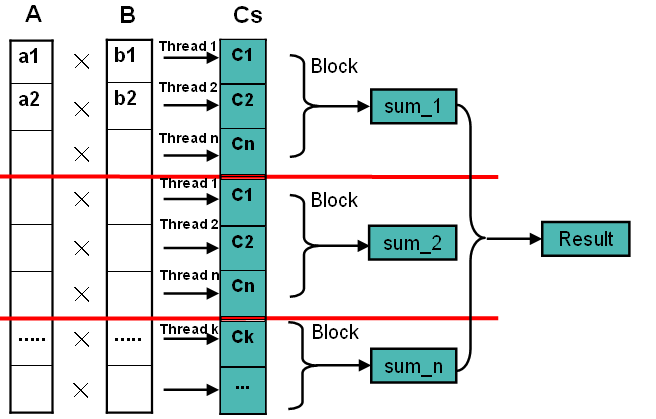
\includegraphics[width=3.5in]{../xby/pic/Vektor}
\caption{Skalaprodukt: Eingabevektoren $ \bf a$ und $ \bf b$, (Zwischen)Ergebnisvektor $ \bf c$}
\label{Vektor}
\end{figure}
%Implementierung_vollmatrize
Multiplikation von Matrize mit Vektor in CUDA Implementierung\\

Beim Wissenschaftlichen Rechen trifft man häufig die Multiplikation von Matritze mit Vektor. In CUDA Implementierung wird die Oparation als unterschiedliche Vektor-Multiplicationen zerlegt.Mit änlichem Methode werden auch Matizen mit Vektoren multipliziert. Im folgendem Bild Fig.\ref{MatrixVektor}.zeigt, dass jede zerlegte Vektor von A mit Vektor B in einem Block multipliziert wird. 

\begin{figure}[htbp]
%\centering
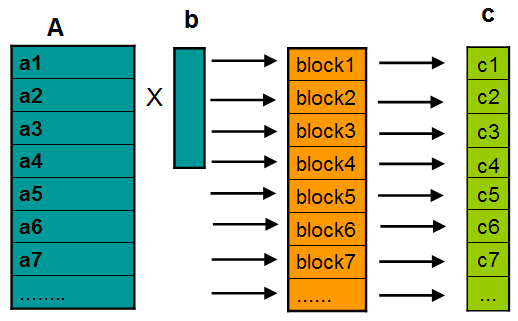
\includegraphics[width=3.5in]{.//pic//MatrixVektor}
\caption{Matrize mal Vektor. A: Matrize; b: Vektor; c: Produktvektor}
\label{MatrixVektor} 
\end{figure}
%Implementierung_sparematrize

%\subsubsection{Sparse Matrix und Vektormultiplikation}
\subsubsection{Matrix-Vektorprodukt mit Sparsematrix}

%sparse_matrize

%Sparsematrix, oder dünnbesetzte Matrix,  bezeichnet man als eine Matrix, bei der so viele Einträge aus Nullen bestehen. Im Abb.\ref{fig:Sparse_Matrix} wird ein einfaches Beispiel gezeigt.
%Da Sparsematrix mit Vollmatrix genau umgekehrt ist, hat man dafür auch eine andere Speicherweise. Unter dem Zusammenhang zwischen Abb.\ref{fig:orignal_sparse}., Abb.\ref{fig:numerische_sparse1}. und Abb.\ref{fig:numerische_sparse2}. versteht man, dass bei der Sparsematrizen wird nun nur die Nonzero-Elemente und die zugehörigen Stelleinformationen(Zeilen und Spalte) gespeichert. Vektor $pr$ enthält alle Nonzero-Elemente. Die Vektoren $ir$ und $jc$ enthalten die Zeileninformation und die Spalteinformation. Im Abb.\ref{fig:numerische_sparse2}. bezeichnet man, wie die Informationen gepackt werden. Die Werte von $jc[i]$ und $jc[i+1]-1$ zeigen den Indexe, deren die zur Spalte $i$  gehörteten Nonzero-Elemente und Zeileinformation aufweisen.

Als Sparsematrix oder dünnbesetzte Matrix bezeichnet man eine
Matrix bei der die Mehrheit der Elemente aus Nullen besteht.
Abb.\ref{fig:Sparse_Matrix} zeigt von links
nach rechts die Reduktion von einer vollbesetzten Struktur
zu einer platzsparenden Struktur.
Aus Platzspargründen nutzt Matlab ein spezielles Memorylayout \cite{matlabsparse}
mit dem nur die nonzero-Elemente im Speicher gehalten werden.

%\begin{figure}[htbp]
%	\includegraphics[width=1in]{.//pic//orignal_sparse}
%	\caption{Original-Matrize}
%	\includegraphics[width=1in]{.//pic//numerische_sparse1}
%	\caption{Sparsame Struktur}
%	\includegraphics[width=1in]{.//pic//numerische_sparse2}
%	\caption{compressed column structure"}
%\end{figure}

% \begin{figure}[htbp]
	% \begin{center}
		% \begin{minipage}[t]{0.4\linewidth}
			% \centering
			% \includegraphics[width=\linewidth]{../xby/pic/orignal_sparse}
			% \caption{Original-Matrize}
			% \label{orignal_sparse}
		% \end{minipage}
		% \qquad
		% \begin{minipage}[t]{0.4\linewidth}
			% \centering
			% \includegraphics[width=\linewidth]{../xby/pic/numerische_sparse1}
			% \caption{Sparsame Struktur}
			% \label{numerische_sparse1}
		% \end{minipage}
		% \qquad
		% \begin{minipage}[t]{0.4\linewidth}
			% \centering
			% \includegraphics[width=\linewidth]{../xby/pic/numerische_sparse2}
			% \caption{"compressed column structure"}
			% \label{numerische_sparse2}
		% \end{minipage}
	% \end{center}
% \end{figure}

\begin{figure}[htbp]
  \centering
     \subfloat[][Original-Matrize]{\label{fig:orignal_sparse}\includegraphics[width=2.4cm]{../xby/pic/orignal_sparse}}
	 \hspace{0.5cm}
	\subfloat[][Sparsame Struktur]{\label{fig:numerische_sparse1}\includegraphics[width=2.4cm]{../xby/pic/numerische_sparse1}}
	\hspace{0.5cm}
	\subfloat[]["compressed column structure"]{\label{fig:numerische_sparse2}\includegraphics[width=2.4cm]{../xby/pic/numerische_sparse2}}
  \caption{Sparse Matrix}
  \label{fig:Sparse_Matrix}
\end{figure}


%Mit obengenanntem Methode werden Spasematrizen in Spaltfolg gespeichert. Bei unser Implementierung verwenden wir es als Zeilfolg. Im folgendem Abb.\ref{sparseMul}. zeigt, wie die Multiplikation ausgeführt wird

Unsere CUDA-Implementierung verwendet zur Speicherung ein abgewandeltes
Matlab-Format. Statt in Spaltenfolge speichern wir die Matrix
in Zeilenfolge, um bei der Multiplikation mit einem Spaltenvektor direkt
die Multiplikationsschleife ,,über die Zeile treiben'' zu können.

\begin{figure}[htbp]
%\centering
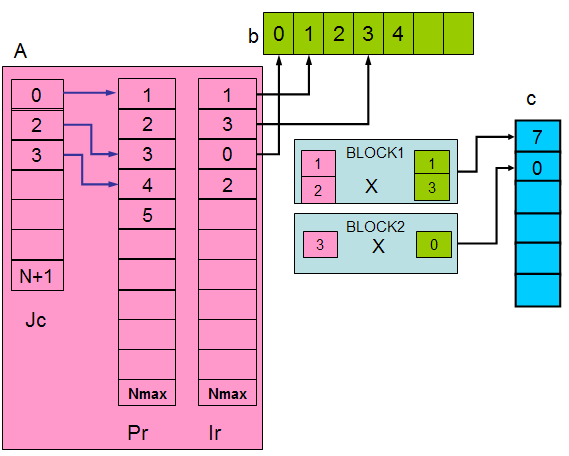
\includegraphics[width=3.5in]{../xby/pic//sparseMul}
\caption{Matrix-Vektorprodukt mit Sparsematrix: Sparsematrix $\bf A $, Zeilenindex $ \bf j_c$, Nonzero-Elemente $\bf j_r$,  Spalteninformation $ \bf I_r$, Multiplikand $\bf b$, Produkt $\bf c$}
\label{sparseMul}
\end{figure}


\subsubsection{Löser Gauss}
Basis für die CUDA Implementierung ist ein Algoritumus aus der
Standardliteratur \cite{sedgewick} mit Pivotisierung.
Da Teile des Algorithmus (Rückwärtssubstitution, Maximum suchen bei der
Povitisierung) nur sequentiell ausgeführt werden können fehlt die volle
Ausnutzung der Parallelität.

% An example of a floating figure using the graphicx package.
% Note that \label must occur AFTER (or within) \caption.
% For figures, \caption should occur after the \includegraphics.
% Note that IEEEtran v1.7 and later has special internal code that
% is designed to preserve the operation of \label within \caption
% even when the captionsoff option is in effect. However, because
% of issues like this, it may be the safest practice to put all your
% \label just after \caption rather than within \caption{}.
%
% Reminder: the "draftcls" or "draftclsnofoot", not "draft", class
% option should be used if it is desired that the figures are to be
% displayed while in draft mode.
%
%\begin{figure}[!t]
%\centering
%\includegraphics[width=2.5in]{myfigure}
% where an .eps filename suffix will be assumed under latex,
% and a .pdf suffix will be assumed for pdflatex; or what has been declared
% via \DeclareGraphicsExtensions.
%\caption{Simulation Results}
%\label{fig_sim}
%\end{figure}

% Note that IEEE typically puts floats only at the top, even when this
% results in a large percentage of a column being occupied by floats.


% An example of a double column floating figure using two subfigures.
% (The subfig.sty package must be loaded for this to work.)
% The subfigure \label commands are set within each subfloat command, the
% \label for the overall figure must come after \caption.
% \hfil must be used as a separator to get equal spacing.
% The subfigure.sty package works much the same way, except \subfigure is
% used instead of \subfloat.
%
%\begin{figure*}[!t]
%\centerline{\subfloat[Case I]\includegraphics[width=2.5in]{subfigcase1}%
%\label{fig_first_case}}
%\hfil
%\subfloat[Case II]{\includegraphics[width=2.5in]{subfigcase2}%
%\label{fig_second_case}}}
%\caption{Simulation results}
%\label{fig_sim}
%\end{figure*}
%
% Note that often IEEE papers with subfigures do not employ subfigure
% captions (using the optional argument to \subfloat), but instead will
% reference/describe all of them (a), (b), etc., within the main caption.


% An example of a floating table. Note that, for IEEE style tables, the
% \caption command should come BEFORE the table. Table text will default to
% \footnotesize as IEEE normally uses this smaller font for tables.
% The \label must come after \caption as always.
%
%\begin{table}[!t]
%% increase table row spacing, adjust to taste
%\renewcommand{\arraystretch}{1.3}
% if using array.sty, it might be a good idea to tweak the value of
% \extrarowheight as needed to properly center the text within the cells
%\caption{An Example of a Table}
%\label{table_example}
%\centering
%% Some packages, such as MDW tools, offer better commands for making tables
%% than the plain LaTeX2e tabular which is used here.
%\begin{tabular}{|c||c|}
%\hline
%One & Two\\
%\hline
%Three & Four\\
%\hline
%\end{tabular}
%\end{table}


% Note that IEEE does not put floats in the very first column - or typically
% anywhere on the first page for that matter. Also, in-text middle ("here")
% positioning is not used. Most IEEE journals use top floats exclusively.
% Note that, LaTeX2e, unlike IEEE journals, places footnotes above bottom
% floats. This can be corrected via the \fnbelowfloat command of the
% stfloats package.



\section{Typische Probleme bei der GPU-Programmierung}


Die besondere Architektur der GPU führt zu besonderen Problemen
und Ansätzen zur Problemlösung.

%Typische Problem  Dreiecksmassig

%In der GPU-Programmierung kann mann auch viele Probleme treffen.

\subsection{Dreieckförmige Summation}
Ein typisches Problem ist Bloksummation. Aus der Beschreibungen der Operationen Multiplikationen der Matrix mal Vektor und Sparsematrize  mal Vektor beruhen obige Operationen auf Vektormultiplikationen, die schließlich ein Summierungsverfahren in jedem Block enthalten. Blocksummation in einzigen Thread ist nicht effizient. Die einführende Algorithmus: Dreieckförmige Summation lautet wie Fig.\ref{Dreieck} . In erst Schritte werden 2n und 2n+1 Elements des Produktvektors $cs$ in jeweilig Threads summiert. In zweiter Schritte werden 4n und 4n+2 Elements summiert. Bis BlockSize/2 Schritte erhalt man endlich Ergebnisse.

\begin{figure}[htbp]
%\centering
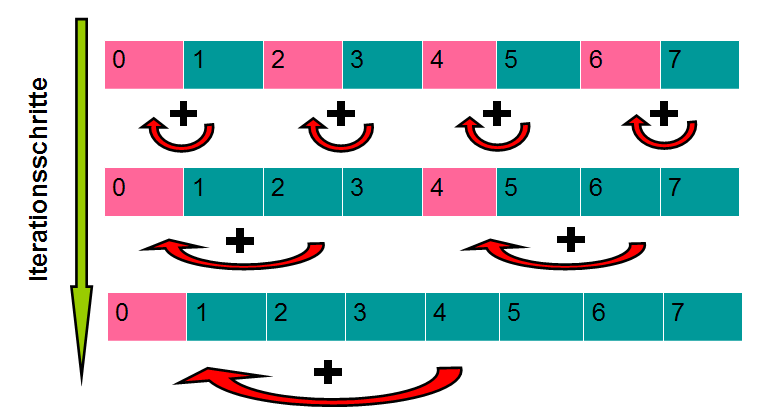
\includegraphics[width=3.5in]{../xby/pic//dreieck}
\caption{\label{Dreieck}Dreieckförmige Summation. Von Oben nach Unter zeigt}
\end{figure}

Beispiel Code kann man in \cite{reduction} finden.

%%Dreieckmassig code zeigen
\begin{verbatim}
#define BLOCK_EXP 9
#define DEF_BLOCKSIZE 1 << BLOCK_EXP
short offset = 1;
for (short i = 1;i < BLOCK_EXP; i++) {
    short old = offset;
    offset <<= 1;
    if (threadIdx.x % offset == 0) {
        Vs[threadIdx.x] += Vs[threadIdx.x
        										+ old];
    }
    __syncthreads();
}
if (threadIdx.x == 0) {
    out[0] = Vs[0] + Vs[offset];
}
\end{verbatim}

%Minimierung leer Thread
\subsection{Minimierung leer laufende Thread}

In CUDA bearbeitet jeder Multiprozessor gleichzeitig mit 32 Threads \cite{cudapg}, die allen zum selben Block gehören. Bei der Sparematrix-Multiplikation sind viele Threads am leerlaufen. Um die Leerlaufenden Threads zu minimieren, müssen mehrere Punktprodukte in einem Block bearbeitet werden. Dazu verwendet man 2 dimensionierte Blocksizes. Die Definition und Anwendung von 2-D Blocksize findet man in der Referenz\cite{cudapg} und \cite{cudbp}. 

% \begin{figure}[htbp]
	% 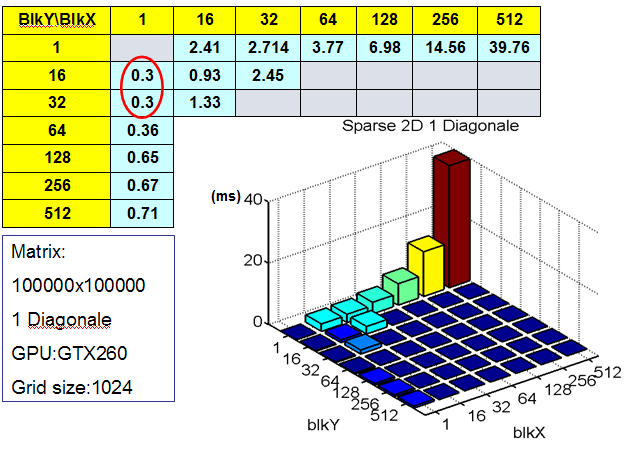
\includegraphics[width=1.7in]{../xby/pic//einDiagonal}
	% \caption{Multipliktion Ein-Diagonalematrize mal Vektor. BlockY: Anzahl der Y-Dimension von Block; BlockX: Anzahl der X-Dimension von Block}
	% 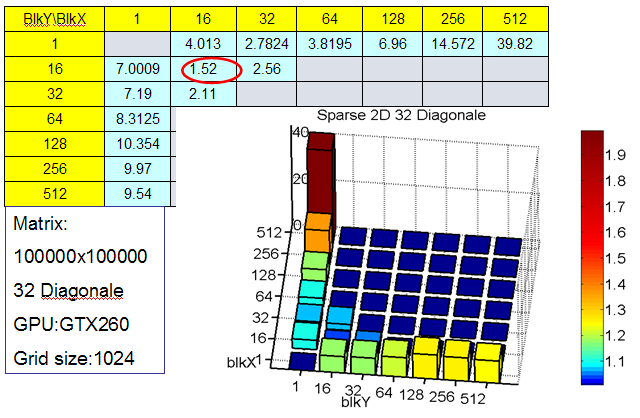
\includegraphics[width=1.7in]{../xby/pic//moreDiagonal}
	% \caption{Multipliktion 32-Diagonalematrize mal Vektor. BlockY: Anzahl der Y-Dimension von Block; BlockX: Anzahl der X-Dimension von Block.}
% \end{figure}
%share memory
\subsection{Shared Memory}
In der Grafikkate ist der Zugriff auf den globalen Speicher langsamer als auf den On-Chip-Speicher.  Wie Beispiele in \cite{cudapg} gezeigt, kann man mehrer mal verwendete Daten zunächst in shared Memory schreiben, dann für die entsprechenden Operationen benutzen. In der Multiplikation der Vollmatrize mal Vektor wird jede Vektorelement mehr mal gebraut. Nach Untersuchungen wählen wir 1-Dimensionblock,die 64 beträgt und jede Vektorelement 8 mal gebraucht in einem Block, d.h. in jedem Block 8 zerlegende Vektormultiplikation bearbeitet werden. Aus den Ergebnisse von Abb.\ref{sharememory}.(Vergleich von optimierte Vollmatrixmultiplikation mit C-Implementierung und alte GPU-Implementirung für MxN Vollmatrizen).
\begin{figure}[htbp]
%\centering
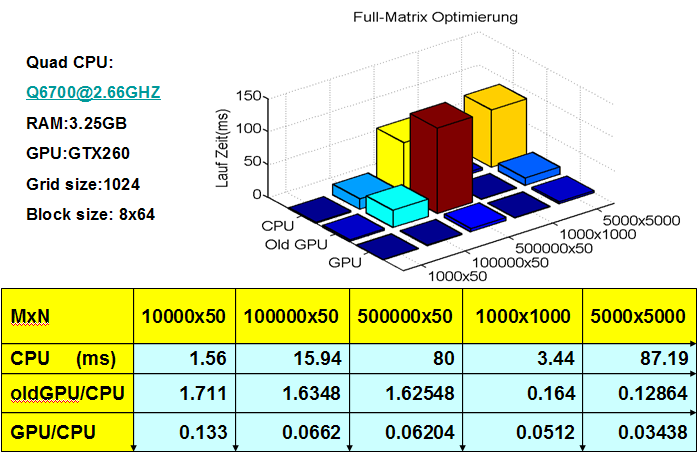
\includegraphics[width=3.5in]{../xby/pic/sharememory}
\caption{Vergleich von optimierte Vollmatrixmultiplikation mit C-Implementierung und alte GPU-Implementirung für $M$ * $N$ Vollmatrix}
\label{sharememory}
\end{figure}


%\usepackage{booktabs}
%\usepackage{tabularx}
\begin{table}
\caption{Ausführungszeiten der Vollmatrixmultiplikation} 
\label{shared_memory}
%\begin{tabular}{|l|c|c|c|c|c|}
\centering
\begin{tabular}{|p{46pt}p{28pt}p{30pt}p{28pt}p{30pt}p{30pt}|}
%\begin{tabularx}{350pt}{1xxxxx}
\toprule
%\hline
	$M$ * $N$& 10000x50& 100000x50& 50000x50& 1000x1000& 5000x5000\\

\midrule
%\hline
CPU(ms)& 1.56&    15.94& 				80&      3.44& 87.9\\

old GPU/CPU& 1.711& 1.6348&   1.62548&  0.164&  0.12854\\

GPU/CPU & 0.133& 0.0662&     0.06204&   0.0512& 0.03438\\
\bottomrule
%\hline     
\end{tabular}
%\end{tabularx}
\end{table}
Die optimierte GPU-Implementierung ist immer schnelle als die CPU-Implementierung  und die Alte. Für Matrix 5000x5000 kann die CUDA-Programm 30 mal schneller als CPU


%Block�bergreifen
\subsection{Blockübergreifende Synchronisation schwierig}
Ein Weiter Problem befindet sich auf der Blocksyncronisation. Für größe Vekotrmultiplkation verwendet man wissentlich mehre Blöcke. Schließlich bekomt man ein Vektor von jede Blocksummer. Da Ohne valide Synchronisationsmaßnahme um alle Blocksummer zu synchronisieren, kann man den Vektor nicht direkt im selbes Kernel bearbeiten. Die mögliche Lösungen stellt da, 1st .die gesammte Summier wird in Cpu ausgerechnet.. 2.man leitet den Vektor von jede Blocksummer zu einem neu Kernel, das sich Summierung beschäftigt.


\subsection{Texture Memory}

Die Karteneinheit für ,,Texture Memory'' kann nicht benutzt werden
zur Beschleunigung weil diese nur float, aber nich double unterstützt.

\subsection{Fehlersuche im laufenden Algorithmus}

Der auf der Karte ablaufende Prozess ist zum Debuggen und
automatisierten Testen zunächst schwer zugänglich weil
die klassischen Instrumente des Debuggings, angefangen beim
klassischen 'printf()' darauf aufsetzen daß alle benötigten Daten
im Speicher zugänglich sind.

Diese Probleme werden in unserer Implementierung adressiert
durch eine Zwischenschicht die im Debugging Mode die jeweils
für das Debugging relevanten Daten aus der Karte extrahiert und
in leicht verarbeitbarer Form ins Memory spiegelt:

Die Einzelnen Operationen werden je in ein Command-Muster \cite{entwurfsmuster} gewrappt
und je einmal in CUDA und auf der Host-CPU implementiert. Die Host-Implemetierung
wird dabei als Referenz und Sollwertgeber für das erwartete Ergebnis benutzt.
Der Algorithmus wurde als Template-Muster ausgeführt so daß im Testbetrieb wahlweise
CUDA-und CPU Operationen auf die Algorithmus-Instanz aufkonfiguriert werden können
oder zwei Algorithmus-Instanzen im Parallelbetrieb gefahren werden können.
Dadurch können wir im Testbetrieb alle Algorithmusschritte mit einem Soll-Ist-Vergleich
durchfahren und so automatisiert jene Abweichungen zwischen CPU-und CUDA-Implementierung lokalisieren die
manuell schwer oder garnicht aufgefunden werden können.


\section{Testergebnisse}

\subsection{sparsemul}

%(buyu)
%sparsemul_result


%Versuch der Vergleichung von matlab,CPU-und GPU-Implementierung wird in Abb.\ref{sparse_ergebnis} und Tabelle \ref{tab_sparse_result}. ausgewiesen. Für 128-Diagonalmatix kann CUDA-Implementierung gegen CPU zu Faktor 9 erreichen.

Der Vergleich von Matlab, CPU- und GPU-Implementierung wird in
Abb.\ref{sparse_ergebnis} und Tabelle \ref{tab_sparse_result} gezeigt.
Für eine 128-Diagonalmatix kann die CUDA-Implementierung (16x16)
einen Speedup-Faktor von 9 gegenüber der CPU erreichen.


\begin{figure}[htbp]
%\centering
%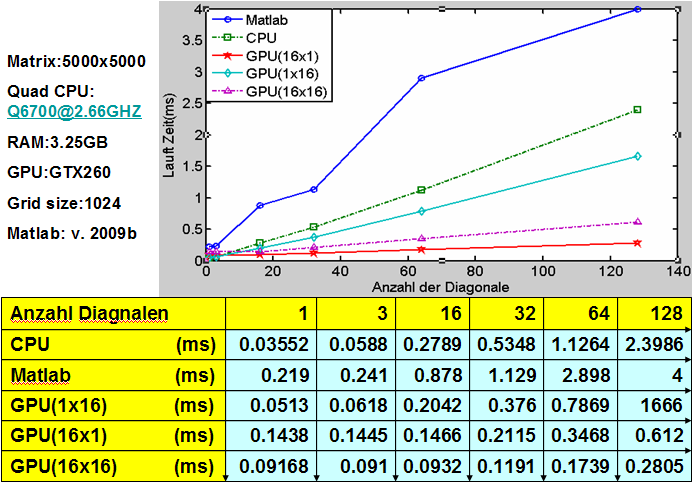
\includegraphics[width=3.5in]{../xby/pic//sparse_ergebnis}
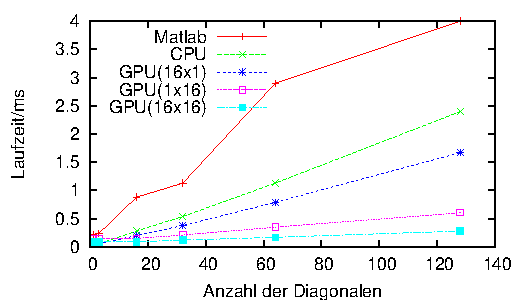
\includegraphics{../ausarbeitung/sparse/sparsegp.pdf}
\caption{Sparsematrix-Vektormultiplikation. Matrix 5000x5000, Quad CPU 2.66GHz, RAM 3.25GB, GPU GTX260, Grid size 1024}
\label{sparse_ergebnis}
\end{figure}


\begin{table}
%\begin{tabular}{|l|c|c|c|c|c|}
\renewcommand{\arraystretch}{1.3}
\caption{Ausführungszeiten der Sparsematrix-Vektormultiplikation in ms}
\label{tab_sparse_result}
\centering
%\begin{tabular}{|p{46pt}p{20pt}p{20pt}p{20pt}p{20pt}p{20pt}p{20pt}|}
\begin{tabular}{|l|r|r|r|r|r|r|}
%\begin{tabularx}{350pt}{1xxxxx}

\hline
Diagonalen& 1& 3& 16& 32& 64 &128\\


\hline
\hline
Matlab     &   0.219   &   0.241&   0.878  &  1.129 &  2.898  & 4\\
CPU        & 	0.036 &   0.059& 	0.279  &  0.535 &  1.126  & 2.399 \\
GPU(1x16)  & 0.051     &   0.062 &  0.204  &  0.376 &  0.787  & 1.666\\
GPU(16x1)  & 0.143     &	0.145 &	0.147  &  0.212 &	0.347 &	0.612\\

GPU(16x16)     & 0.092 &	0.091  &	0.0932 &	0.119&	0.174 &	0.281\\

\hline
\end{tabular}
%\end{tabularx}
\end{table}

\subsection{norm und dotmul}

\begin{figure}[htbp]

   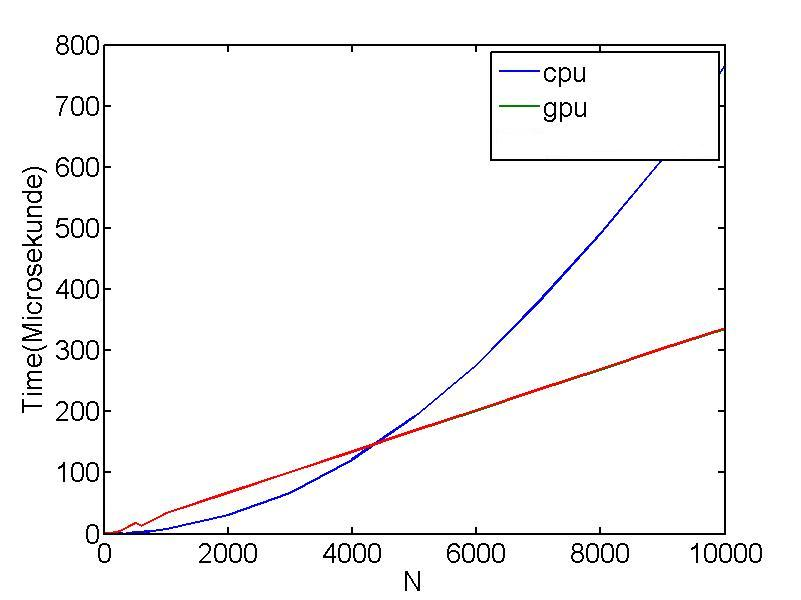
\includegraphics[width=3in]{pix/dotmultime}

   \caption{ \label{dotmultime} Skalarprodukt: Rechenzeit in Abhängigkeit von der Problemgröße }%

\end{figure}


Die Operationen dotmul und Norm laufen für eine Problemgröße $N > 5000$ schneller
als die CPU-Implementierung. (Bild \ref{dotmultime})

Trotz der Standardmaßnahmen \cite{reduction} zur Summierung auf ein Skalar wurde
die Ausführungsszeit nicht schneller als die der CUBLAS-Operationen \cite{cublas}.



\subsection{Löser Gauss}

(tbd Achim) Bislang langsamer als CPU-Implementierung

\subsection{IDR(s) Gesamtalgorithmus}

Testproblem für das Messen ist das LGS für ein 1D-Laplaceproblem mit Randwerten.
Die Zeilenzahl des Test-LGS wird $N$ genannt.

\begin{displaymath}
  \begin{pmatrix}
      2 &  0  &  0  & 0   & 0 \\
      0 &  2  & -1  & 0   & 0 \\
      0 & -1  &  2  & -1  & 0 \\
      0 &  0  &  -1  &  2 & -1 \\
      0 &  0  &  0   &  0 & 2  \\
  \end{pmatrix}
   \cdot \vec{ \bf{x} }
   =
  \begin{pmatrix} 1 \\ 0  \\ 0 \\ 0  \\ -1
  \end{pmatrix}
%a + b
\end{displaymath}


Pro Iterationsschritt $i$ wird das Residuum $r_i = | \bf{A} \cdot \vec{\bf{x_i}} - \vec{b} |$ aufgezeichnet und
im Diagramm \ref{residuum}  gegen $i$ aufgetragen.

Der CUDA-IDR(s) konvergiert bis zu einer Genauigkeit von $10^{-4}$ bei $N=700$

\begin{figure}[htbp]

   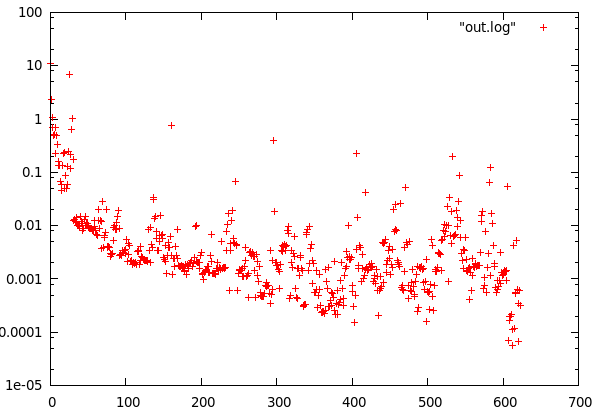
\includegraphics[width=3in]{pix/bastian/image002.png}

   \caption{ \label{residuum} Residuenverlauf des CUDA-IDR(4) bei einer Toleranz von $10^{-4}$ }%

\end{figure}



\section{Möglichkeiten für die weitere Optimierung der IDR(s)-Implementierung}

\begin{itemize}
 \begin{item}
Spezialkernel die angepasst
sind auf bestimmte Matrixgrößen, denn der optimale Kernel für
 $A_{Ns} \cdot B_{s1}$ muß anders implementiert werden als  $A_{sN} \cdot B_{N1}$.
Hier wählt das Operation-Command selbstätigt den passenden Kernel in Abhängigkeit
von s und N.
 \end{item}

\begin{item}

Einfügen von Instrumentation-Code analog dem Tuning-Interface des Oracle-RDBMS \cite{oracle}. Die Idee besteht darin
automatisiert jene Operationen zu identifizieren die in Summe den größten
Beitrag zur Gesamtlaufzeit beitragen.
Das Codeskelett dieses Instrumentation-Codes wurde bereits erstellt,
aber noch nicht im Gesamtsystem verbaut.
\end{item}

\begin{item}
 Operationen-Commands per Regelsatz in Abhängigkeit von Problemgröße und
        Struktur die Größe von Block und Grid wählen
\end{item}
\end{itemize}


\section{Zusammenfassung}



% if have a single appendix:
%\appendix[Proof of the Zonklar Equations]
% or
%\appendix  % for no appendix heading
% do not use \section anymore after \appendix, only \section*
% is possibly needed

% use appendices with more than one appendix
% then use \section to start each appendix
% you must declare a \section before using any
% \subsection or using \label (\appendices by itself
% starts a section numbered zero.)
%


%\appendices
%\section{Proof of the First Zonklar Equation}
%Appendix one text goes here.

% you can choose not to have a title for an appendix
% if you want by leaving the argument blank
%\section{}
%Appendix two text goes here.


% use section* for{reduction} acknowledgement
%\section*{Acknowledgment}
%
%
%The authors would like to thank...


% Can use something like this to put references on a page
% by themselves when using endfloat and the captionsoff option.
\ifCLASSOPTIONcaptionsoff
  \newpage
\fi



% trigger a \newpage just before the given reference
% number - used to balance the columns on the last page
% adjust value as needed - may need to be readjusted if
% the document is modified later
%\IEEEtriggeratref{8}
% The "triggered" command can be changed if desired:
%\IEEEtriggercmd{\enlargethispage{-5in}}

% references section

% can use a bibliography generated by BibTeX as a .bbl file
% BibTeX documentation can be easily obtained at:
% http://www.ctan.org/tex-archive/biblio/bibtex/contrib/doc/
% The IEEEtran BibTeX style support page is at:
% http://www.michaelshell.org/tex/ieeetran/bibtex/
%\bibliographystyle{IEEEtran}
% argument is your BibTeX string definitions and bibliography database(s)
%\bibliography{IEEEabrv,../bib/paper}
%
% <OR> manually copy in the resultant .bbl file
% set second argument of \begin to the number of references
% (used to reserve space for the reference number labels box)
\begin{thebibliography}{1}

\bibitem{idrs}
 Peter Sonneveld and Martin B. van Gijzen, \emph{IDR(s): a family of simple and fast algorithms for solving large nonsymmetric linear systems.}\hskip 1em plus
  0.5em minus 0.4em\relax SIAM J. Sci. Comput. Vol. 31, No. 2, pp. 1035-1062 (2008)



\bibitem{cudapg}
   NVIDIA Corporation. (2009) \emph{ NVIDIA CUDA Programming Guide Version 2.3 }\hskip 1em plus
  0.5em minus 0.4em\relax
[Online] Available: http://www.nvidia.de/object/cuda\_develop\_emeai.html

\bibitem{idrsm}
 Peter Sonneveld and Martin B. van Gijzen, (December 2008) \emph{ idrs.m }\hskip 1em plus
  0.5em minus 0.4em\relax [Online] Available: http://ta.twi.tudelft.nl/NW/users/gijzen/idrs.m



\bibitem{matlabsparse}
   The Math works \emph { Matlab data } \hskip 1em plus
  0.5em minus 0.4em\relax
[Online] Available: http://www.mathworks.com/access/helpdesk/help/techdoc/matlab\_external/f21585.html



\bibitem{cublas}
   NVIDIA Corporation. (2009) \emph{ CUDA CUBLAS } in \emph { CUDA Toolkit v2.3 } \hskip 1em plus
  0.5em minus 0.4em\relax
[Online] Available: http://www.nvidia.de/object/cuda\_develop\_emeai.html





\bibitem{cudbp}
   NVIDIA Corporation. (2009)
  \emph{ NVIDIA CUDA C Programming Best Practices Guide } \hskip 1em plus
  0.5em minus 0.4em\relax CUDA Toolkit 2.3
[Online] Available: http://www.nvidia.de/object/cuda\_develop\_emeai.html



\bibitem{entwurfsmuster}

 Erich Gamma, Richard Helm, Ralph E. Johnson, John Vlissides
  \emph{ Design Patterns. Elements of Reusable Object-Oriented Software.  }\hskip 1em plus
  0.5em minus 0.4em\relax Addison Wesley, 1995


\bibitem{sedgewick}

 Robert Sedgewick
  \emph{ Algorithmen in C  }\hskip 1em plus
  0.5em minus 0.4em\relax Addison Wesley, 1992


\bibitem{oracle}

  Mogens Norgaard
  \emph{ You probably dont't tune right } in
  \emph{ Oracle Insights: Tales of the Oak Table }\hskip 1em plus
  0.5em minus 0.4em\relax New York, Apress, 2004, ch.2, pp 71-94



\bibitem{reduction}
   Mark Harris \emph{ Optimizing Parallel Reduction in CUDA } in \emph{CUDA SDK} \hskip 1em plus
  0.5em minus 0.4em\relax Nvidia Corporation
[Online] Available: http://developer.download.nvidia.com/compute/cuda/1\_1/Website/projects/reduction/doc/reduction.pdf




\end{thebibliography}

% biography section
%
% If you have an EPS/PDF photo (graphicx package needed) extra braces are
% needed around the contents of the optional argument to biography to prevent
% the LaTeX parser from getting confused when it sees the complicated
% \includegraphics command within an optional argument. (You could create
% your own custom macro containing the \includegraphics command to make things
% simpler here.)
%\begin{biography}[{\includegraphics[width=1in,height=1.25in,clip,keepaspectratio]{mshell}}]{Michael Shell}
% or if you just want to reserve a space for a photo:



% You can push biographies down or up by placing
% a \vfill before or after them. The appropriate
% use of \vfill depends on what kind of text is
% on the last page and whether or not the columns
% are being equalized.

%\vfill

% Can be used to pull up biographies so that the bottom of the last one
% is flush with the other column.
%\enlargethispage{-5in}



% that's all folks
\end{document}


